% !TEX TS-program = pdflatex
% !TEX encoding = UTF-8 Unicode

% This is a simple template for a LaTeX document using the "article" class.
% See "book", "report", "letter" for other types of document.

\documentclass[11pt]{article} % use larger type; default would be 10pt

\usepackage[utf8]{inputenc} % set input encoding (not needed with XeLaTeX)
\usepackage[spanish]{babel}

%%% Examples of Article customizations
% These packages are optional, depending whether you want the features they provide.
% See the LaTeX Companion or other references for full information.

%%% PAGE DIMENSIONS
\usepackage{geometry} % to change the page dimensions
\geometry{a4paper} % or letterpaper (US) or a5paper or....
% \geometry{margin=2in} % for example, change the margins to 2 inches all round
% \geometry{landscape} % set up the page for landscape
%   read geometry.pdf for detailed page layout information

\usepackage{graphicx} % support the \includegraphics command and options
\usepackage[outdir=./]{epstopdf}
% \usepackage[parfill]{parskip} % Activate to begin paragraphs with an empty line rather than an indent
\usepackage{listings}

%%% PACKAGES
\usepackage{booktabs} % for much better looking tables
\usepackage{array} % for better arrays (eg matrices) in maths
\usepackage{paralist} % very flexible & customisable lists (eg. enumerate/itemize, etc.)
\usepackage{verbatim} % adds environment for commenting out blocks of text & for better verbatim
%\usepackage{subfig} % make it possible to include more than one captioned figure/table in a single float
\usepackage{subcaption}
\usepackage{url}
\usepackage{diagbox}
\usepackage{amsmath}
\usepackage{pdfpages}
% These packages are all incorporated in the memoir class to one degree or another...

%%% HEADERS & FOOTERS
\usepackage{fancyhdr} % This should be set AFTER setting up the page geometry
\pagestyle{fancy} % options: empty , plain , fancy
\renewcommand{\headrulewidth}{0pt} % customise the layout...
\lhead{}\chead{}\rhead{}
\lfoot{}\cfoot{\thepage}\rfoot{}

%%% SECTION TITLE APPEARANCE
\usepackage{sectsty}
\allsectionsfont{\sffamily\mdseries\upshape} % (See the fntguide.pdf for font help)
% (This matches ConTeXt defaults)

%%% ToC (table of contents) APPEARANCE
\usepackage[nottoc,notlof,notlot]{tocbibind} % Put the bibliography in the ToC
\usepackage[titles,subfigure]{tocloft} % Alter the style of the Table of Contents
\renewcommand{\cftsecfont}{\rmfamily\mdseries\upshape}
\renewcommand{\cftsecpagefont}{\rmfamily\mdseries\upshape} % No bold!

%%% END Article customizations

%%% The "real" document content comes below...

\title{CLP Lab 6 Report}
\author{Albert Aparicio Isarn\\
	\url{albert.aparicio.isarn@alu-etsetb.upc.edu}
	\and
	Héctor Esteban Cabezos\\
	\url{hect.esteban@gmail.com}}
\date{} % Activate to display a given date or no date (if empty),
         % otherwise the current date is printed

\begin{document}

	% ---- MATLAB Code definitions ----- %
	\definecolor{mygreen}{rgb}{0,0.6,0}
	\definecolor{mygray}{rgb}{0.5,0.5,0.5}
	\definecolor{mymauve}{rgb}{0.58,0,0.82}

	\lstset{ %
		%backgroundcolor=\color{white},   % choose the background color; you must add \usepackage{color} or \usepackage{xcolor}
		basicstyle=\ttfamily\footnotesize,        % the size of the fonts that are used for the code
		breakatwhitespace=false,         % sets if automatic breaks should only happen at whitespace
		breaklines=true,                 % sets automatic line breaking
		captionpos=b,                    % sets the caption-position to bottom
		commentstyle=\color{mygreen},    % comment style
		deletekeywords={...},            % if you want to delete keywords from the given language
		escapeinside={\%*}{*)},          % if you want to add LaTeX within your code
		extendedchars=true,              % lets you use non-ASCII characters; for 8-bits encodings only, does not work with UTF-8
		%frame=single,	                   % adds a frame around the code
		keepspaces=true,                 % keeps spaces in text, useful for keeping indentation of code (possibly needs columns=flexible)
		keywordstyle=\color{blue},       % keyword style
		language=Matlab,                 % the language of the code
		otherkeywords={*,...},            % if you want to add more keywords to the set
		%numbers=left,                    % where to put the line-numbers; possible values are (none, left, right)
		%numbersep=5pt,                   % how far the line-numbers are from the code
		%numberstyle=\tiny\color{mygray}, % the style that is used for the line-numbers
		rulecolor=\color{black},         % if not set, the frame-color may be changed on line-breaks within not-black text (e.g. comments (green here))
		showspaces=false,                % show spaces everywhere adding particular underscores; it overrides 'showstringspaces'
		showstringspaces=false,          % underline spaces within strings only
		showtabs=false,                  % show tabs within strings adding particular underscores
		stepnumber=2,                    % the step between two line-numbers. If it's 1, each line will be numbered
		stringstyle=\color{mymauve},     % string literal style
		tabsize=2,	                   % sets default tabsize to 2 spaces
		title=\lstname                   % show the filename of files included with \lstinputlisting; also try caption instead of title
	}

\maketitle

\section{Preparación de la base de datos}

\begin{figure}[h]
	\centering
	\begin{subfigure}[b]{0.435\textwidth}
		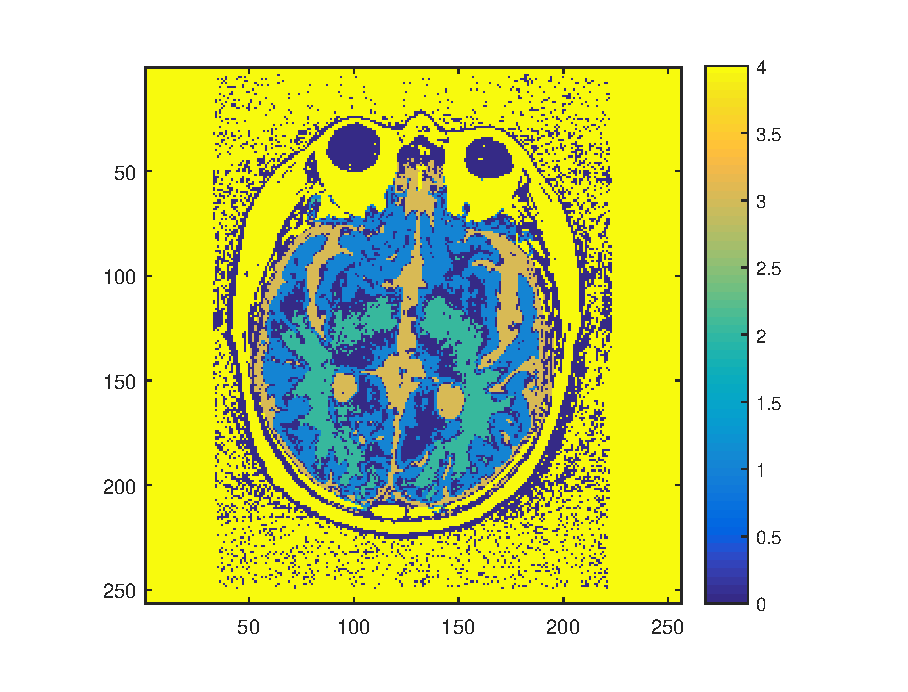
\includegraphics[width=\textwidth]{../1_DB/labels_075.eps}
		\caption[]{\small $P_{min} = 0.75$}
		\label{fig:db:075}
	\end{subfigure}
	\quad
	\begin{subfigure}[b]{0.435\textwidth}
		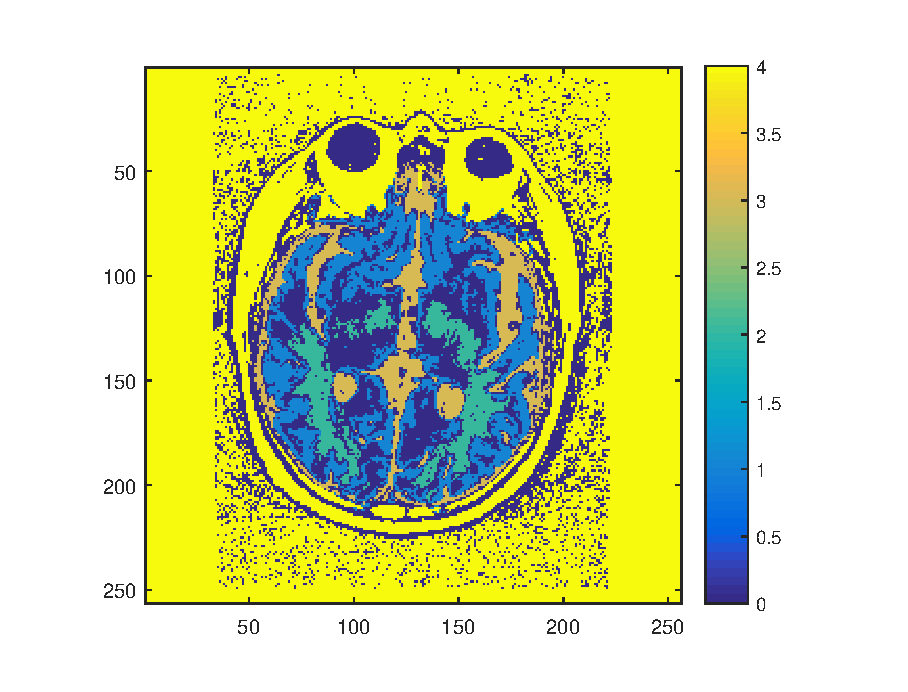
\includegraphics[width=\textwidth]{../1_DB/labels_085.eps}
		\caption[]{\small $P_{min} = 0.85$}
		\label{fig:db:085}
	\end{subfigure}
	\vskip\baselineskip
	\begin{subfigure}[b]{0.435\textwidth}
		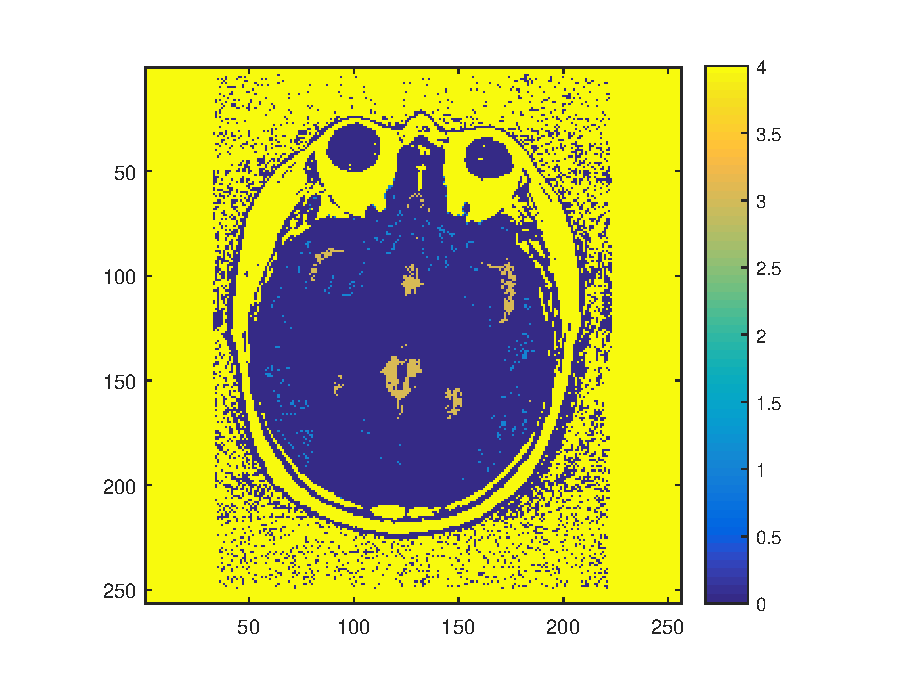
\includegraphics[width=\textwidth]{../1_DB/labels_1.eps}
		\caption[]{\small $P_{min} = 1$}
		\label{fig:db:100}
	\end{subfigure}
	\caption{Imagenes resultantes de las labels con varios valores de $P_{min}$}
	\label{fig:db}
\end{figure}

La elección de $P_{min}$ determina la cantidad de píxeles que se marcan como no
pertenecientes a ninguna clase. Estos píxeles se marcan como tales porque su
probabilidad es menor a $P_{min}$.

A medida que se aumenta $P_{min}$, aumenta el número de estos píxeles, aunque el
resto de píxeles son más "fiables", ya que tienen mayor probabilidad.

Por tanto, se debe encontrar un compromiso entre la fiabilidad de la decisión
y el número de píxeles no clasificados.

\section{Neural networks}

\subsection{Clasificación con Back-Propagation}

Usando este algoritmo, la clasificación da las siguientes probabilidades de error:

\begin{align}
P_{e_{train}} &= 0.0190581 \\
P_{e_{validation}} &= 0.0207211 \\
P_{e_{test}} &= 0.0178201
\end{align}

Los resultados de la clasificación se muestran en la figura \ref{fig:nn:backprop}.

\begin{figure}%[h]
	\centering
	\begin{subfigure}[b]{0.435\textwidth}
		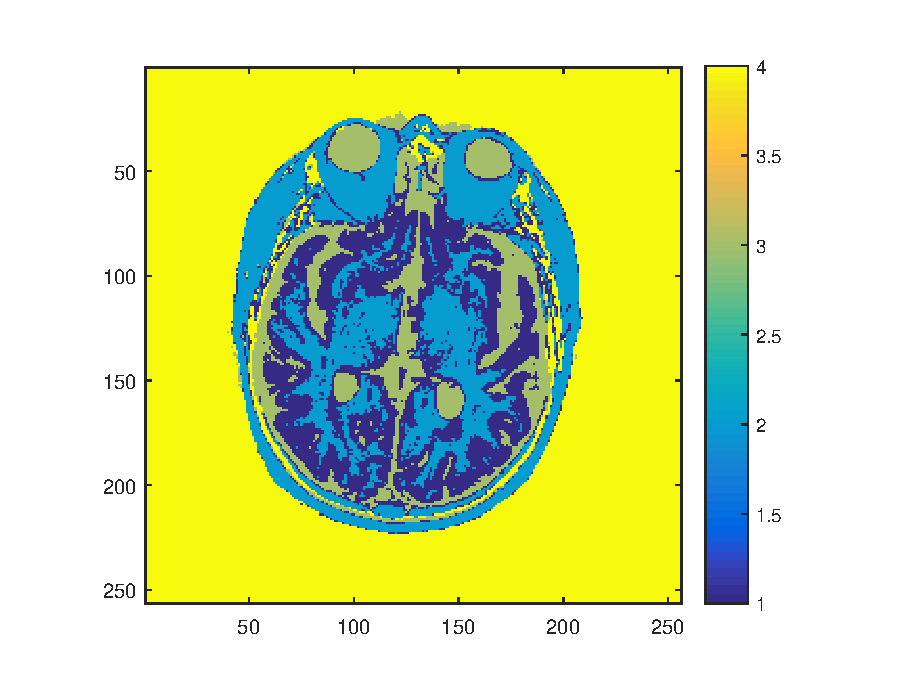
\includegraphics[width=\textwidth]{../2_NN/class_backprop_100000.eps}
		\caption[]{\small Resultado de la clasificación}
		\label{fig:nn:backprop:class}
	\end{subfigure}
	\quad
	\begin{subfigure}[b]{0.435\textwidth}
		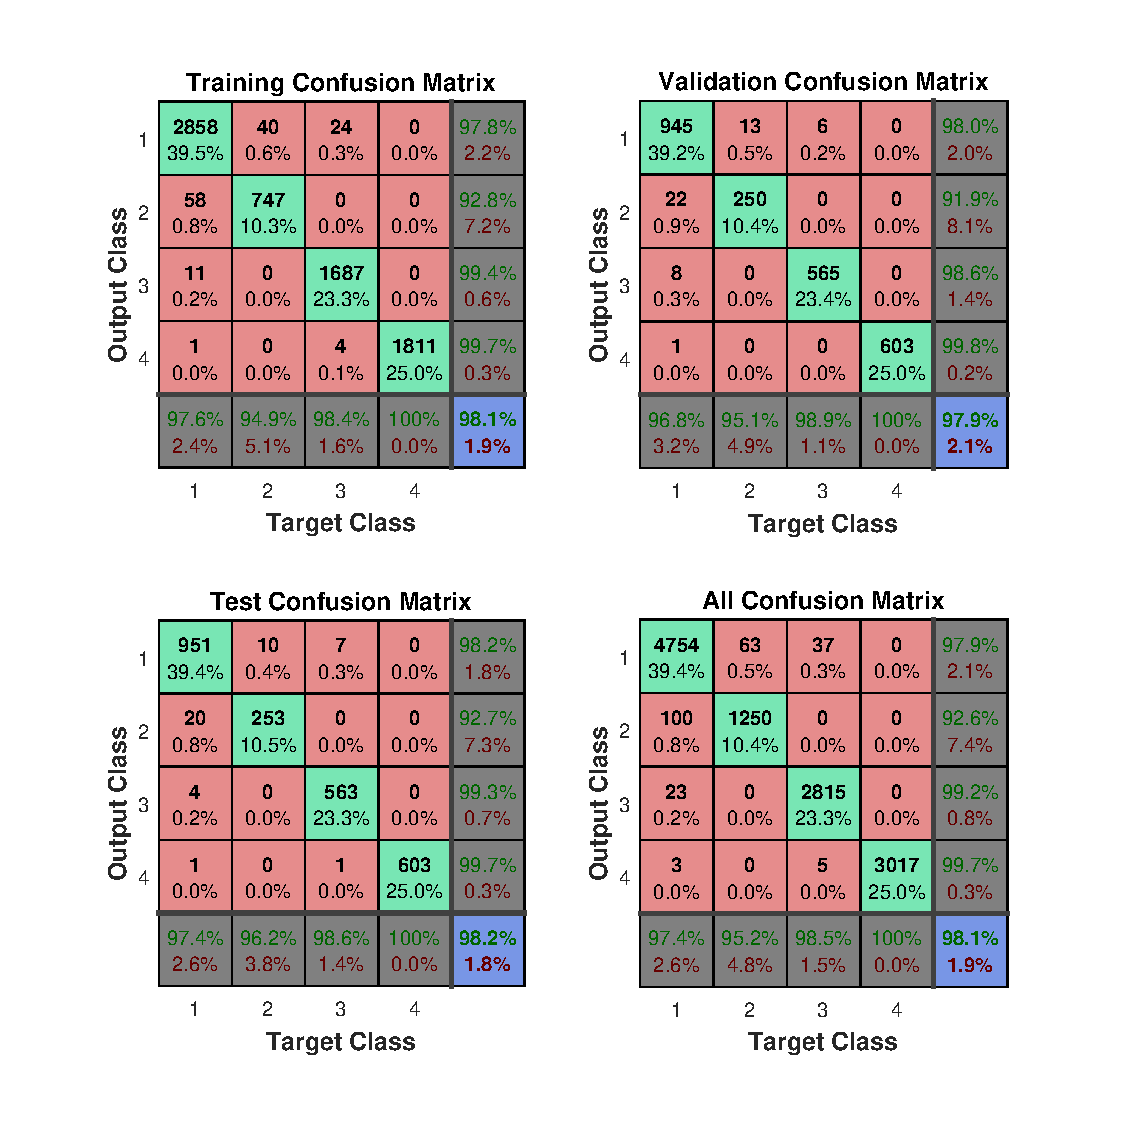
\includegraphics[width=\textwidth]{../2_NN/conf_backprop_100000.eps}
		\caption[]{\small Matriz de confusión}
		\label{fig:nn:backprop:conf}
	\end{subfigure}
	\vskip\baselineskip
	\begin{subfigure}[b]{0.435\textwidth}
		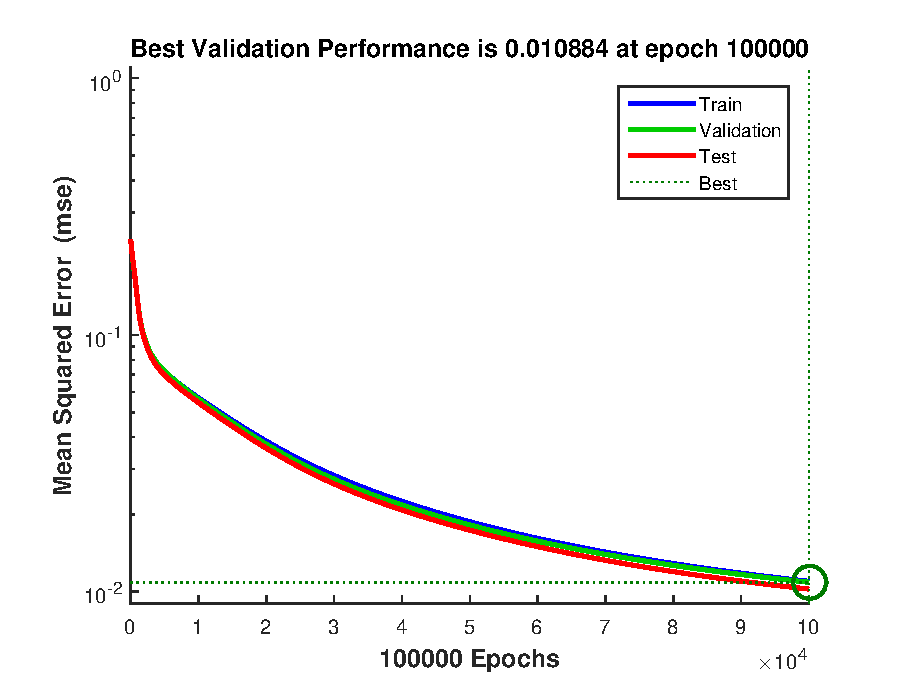
\includegraphics[width=\textwidth]{../2_NN/perf_backprop_100000.eps}
		\caption[]{\small Gráfico de \emph{losses} según cada época}
		\label{fig:nn:backprop:perf}
	\end{subfigure}
	\caption{Resultados de la clasificación con Back-Propagation con 100000 \emph{epochs}.}
	\label{fig:nn:backprop}
\end{figure}

\subsection{Clasificación con Levenberg-Marquadt}

Usando este algoritmo, la clasificación da las siguientes probabilidades de error:

\begin{align}
P_{e_{train}} &= 0.00124292 \\
P_{e_{validation}} &= 0.00207211 \\
P_{e_{test}} &= 0.00414422
\end{align}

Los resultados de la clasificación se muestran en la figura \ref{fig:nn:leven}. En la figura \ref{fig:nn:leven:perf} se ve claramente como el pendiente de las curvas de error es mayor, además de que el algoritmo se detiene a las 32 épocas. Claramente la convergencia de este algoritmo es mucho más rápida que la de Back-Propagation.

\begin{figure}%[h]
	\centering
	\begin{subfigure}[b]{0.435\textwidth}
		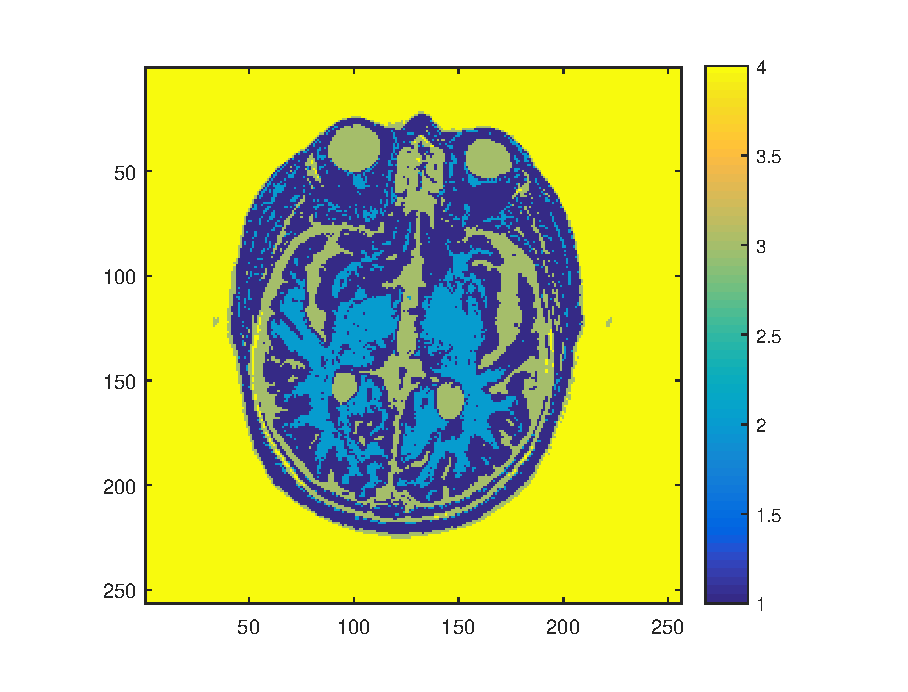
\includegraphics[width=\textwidth]{../2_NN/class_leven_32.eps}
		\caption[]{\small Resultado de la clasificación}
		\label{fig:nn:leven:class}
	\end{subfigure}
	\quad
	\begin{subfigure}[b]{0.435\textwidth}
		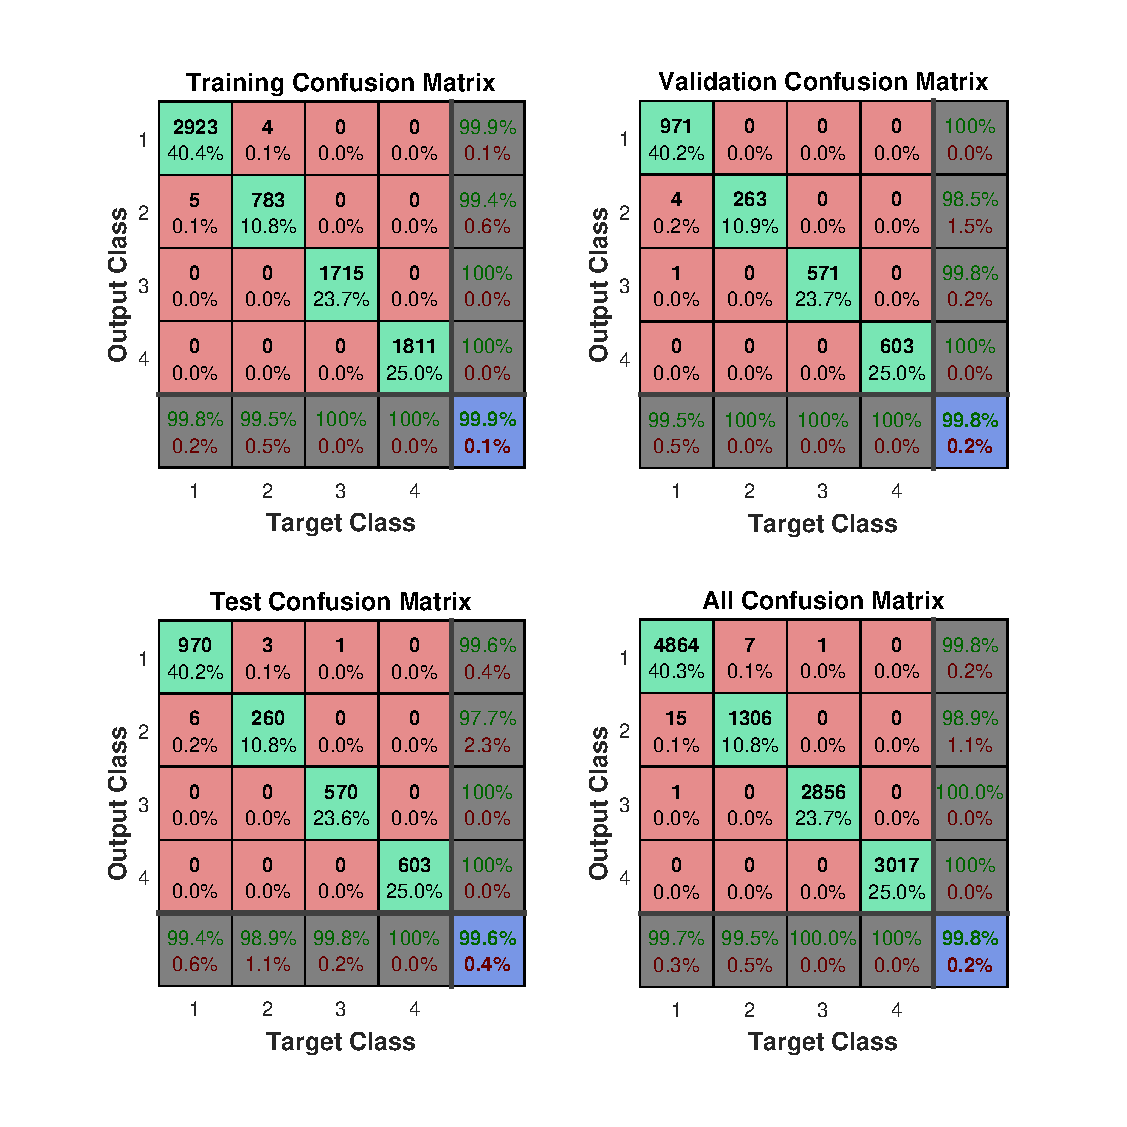
\includegraphics[width=\textwidth]{../2_NN/conf_leven_32.eps}
		\caption[]{\small Matriz de confusión}
		\label{fig:nn:leven:conf}
	\end{subfigure}
	\vskip\baselineskip
	\begin{subfigure}[b]{0.435\textwidth}
		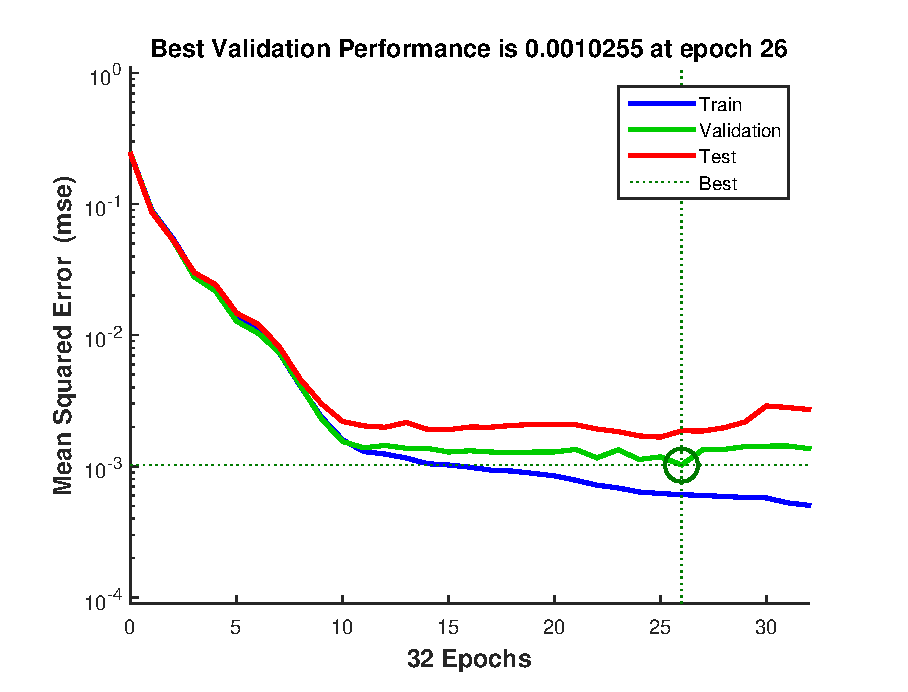
\includegraphics[width=\textwidth]{../2_NN/perf_leven_32.eps}
		\caption[]{\small Gráfico de \emph{losses} según cada época}
		\label{fig:nn:leven:perf}
	\end{subfigure}
	\caption{Resultados de la clasificación con Levenberg-Marquadt con 32 \emph{epochs}.}
	\label{fig:nn:leven}
\end{figure}

\subsection{Comparación de los algoritmos}

El algoritmo de Levenberg-Marquadt proporciona una convergencia más rápida, con menor probabilidad de error, que el algoritmo de Back-Propagation.

Para este problema se podría decir que el algoritmo de Levenberg-Marquadt es más adecuado.

\newpage

\subsection{Validación del número de neuronas a utilizar}

Según los resultados de las varias clasificaciones, el número óptimo de unidades en la red es de \textbf{14}.

Con este tamaño de capa, el error obtenido en test es de $P_{e_{test}} = 0.00248653$.

El código usado para esta sección se muestra a continuación:

\lstinputlisting{2_NN_val_opt.m}

\newpage

\section{Decision trees}

La clasificación ha dado como resultado las siguientes probabilidades de error:

\begin{align}
P_{e_{train}} &= 0.00234774 \\
P_{e_{validation}} &= 0.00828844 \\
P_{e_{test}} &= 0.00828844
\end{align}

A continuación se muestran las matrices de confusión obtenidas para entrenamiento, validación y test, respectivamente:

\begin{equation} \label{eq:tree:train}
\left( \begin{array}{cccc}
2922 &   6 &    0 &    0 \\
11 & 776 &    0 &    0 \\
0 &   0 & 1715 &    0 \\
0 &   0 &    0 & 1811 \\ 
\end{array} \right)
\end{equation}

\begin{equation} \label{eq:tree:validation}
\left( \begin{array}{cccc}
968 &   7 &   1 &   0 \\
12 & 251 &   0 &   0 \\
0 &   0 & 571 &   0 \\
0 &   0 &   0 & 603 \\
\end{array} \right)
\end{equation}

\begin{equation} \label{eq:tree:test}
\left( \begin{array}{cccc}
971 &   5 &   0 &   0 \\
15 & 248 &   0 &   0 \\
0 &   0 & 571 &   0 \\
0 &   0 &   0 & 603 \\
\end{array} \right)
\end{equation}

El resultado de la clasificación, y el árbol obtenido se muestran en la figura \ref{fig:tree}.

\begin{figure}[h]
	\centering
	\begin{subfigure}[b]{0.435\textwidth}
		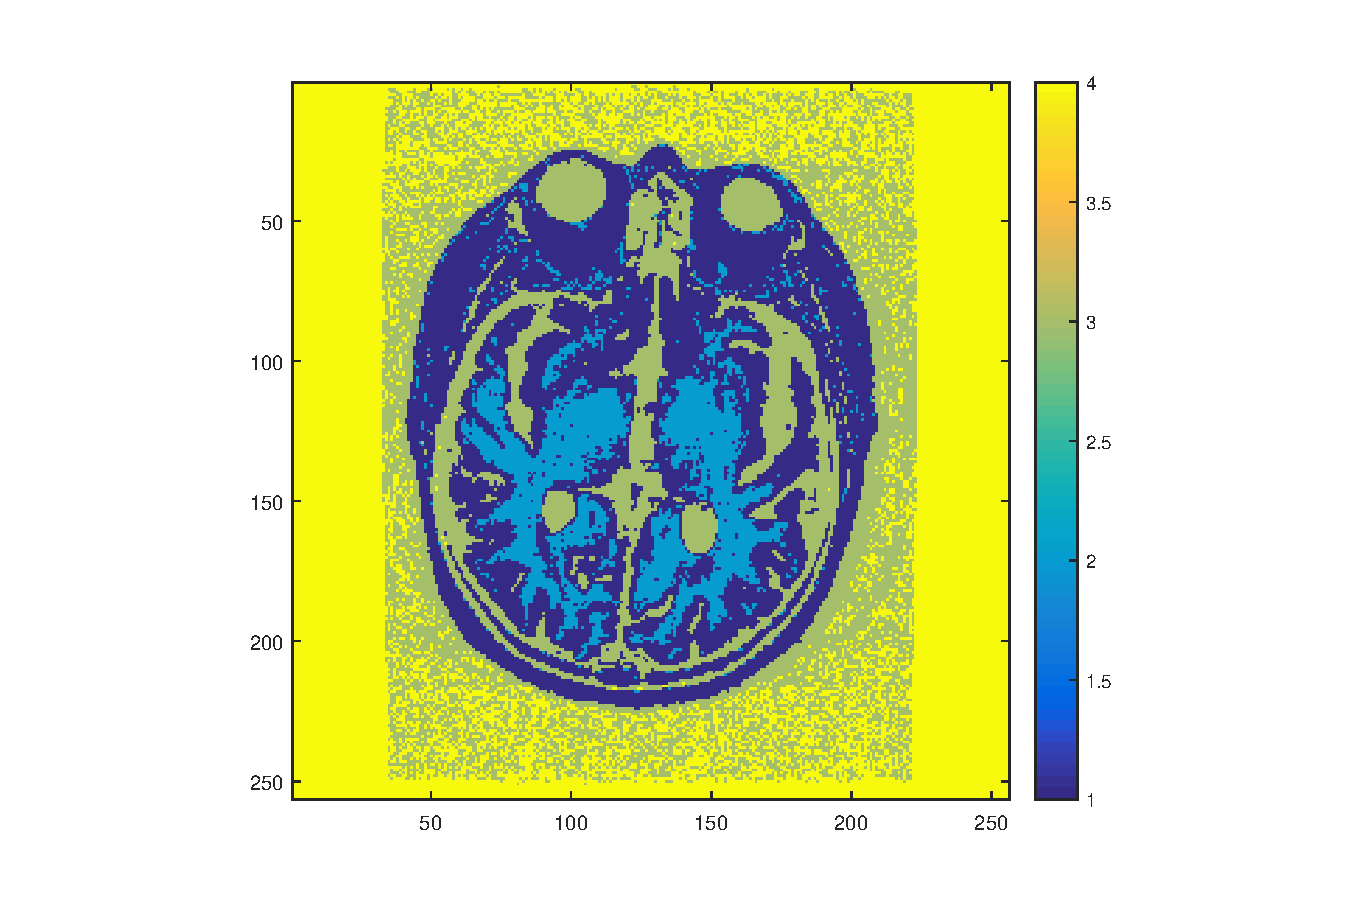
\includegraphics[width=\textwidth]{../3_TREE/1_classification.eps}
		\caption[]{\small Resultado de la clasificación}
		\label{fig:tree:class}
	\end{subfigure}
	\quad
	\begin{subfigure}[b]{0.435\textwidth}
		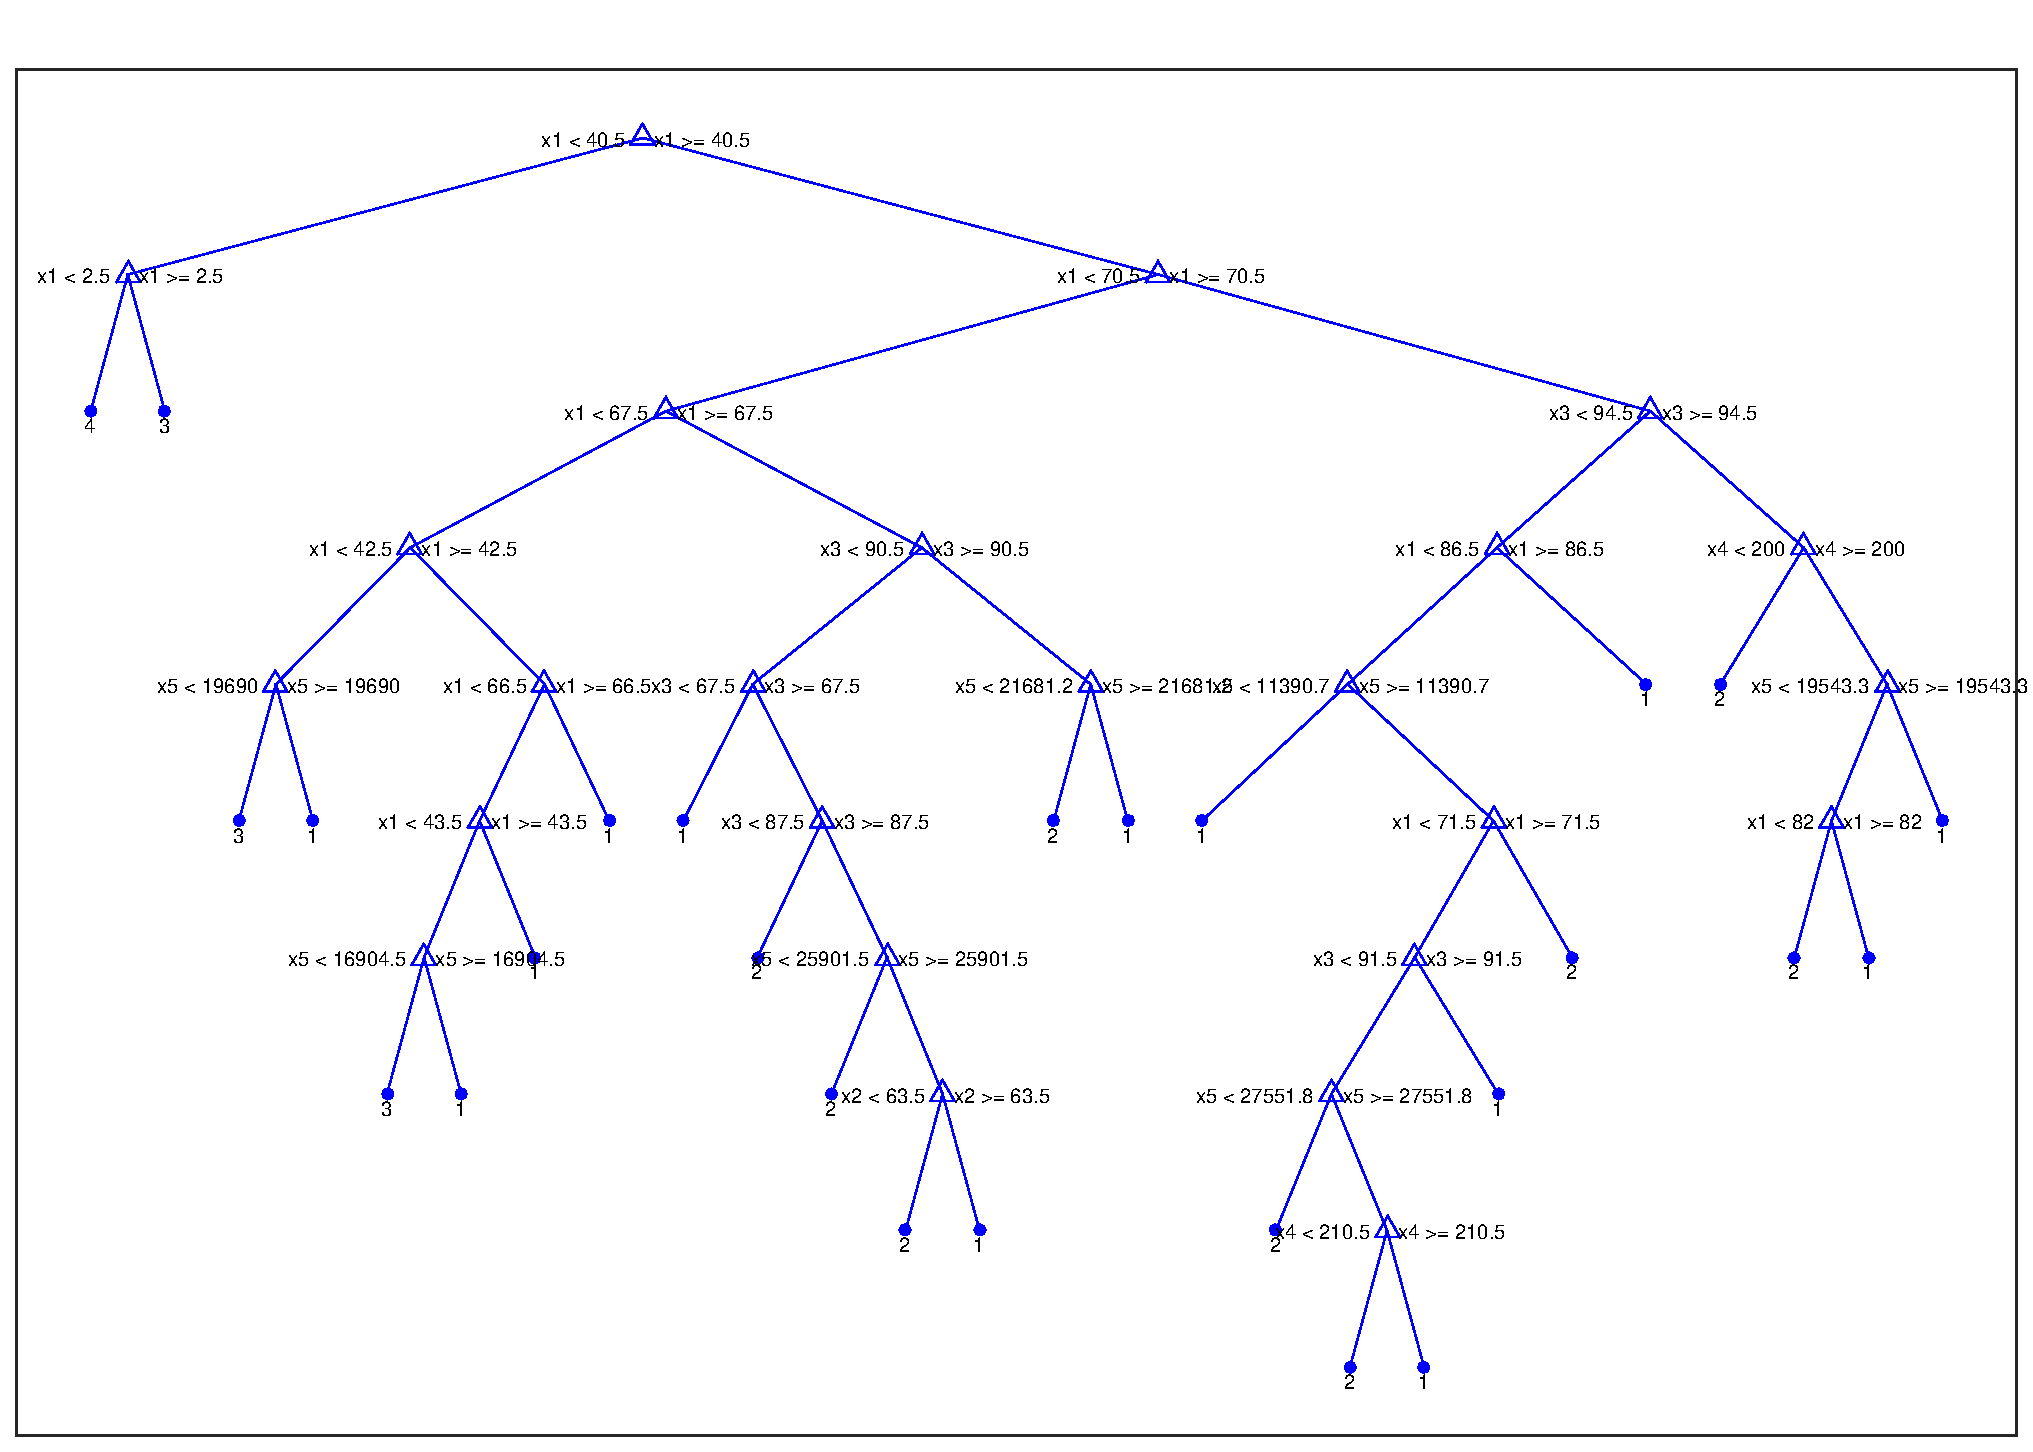
\includegraphics[width=\textwidth]{../3_TREE/1_tree.eps}
		\caption[]{\small Árbol obtenido con el entrenamiento}
		\label{fig:tree:conf}
	\end{subfigure}
	\caption{Resultados de la clasificación con árboles de decisión.}
	\label{fig:tree}
\end{figure}

\newpage

En comparación con el resultado de la red neuronal, el árbol de decisión da un resultado menos preciso y más ruidoso que la red.

\subsection{Validación del número de \emph{splits}}

El número de \emph{splits} óptimo es \textbf{25}. El error de test en este caso es de $P_{e_{test}} = 0.00663075$.

El código generado para esta sección se muestra a continuación:

\lstinputlisting{3_TREE_val_opt.m}

La clasificación es más precisa con redes neuronales, aunque su entrenamiento sea más costoso computacionalmente y lento.	

\section{Clasificación de una imagen nueva}

La clasificación con árboles resulta ruidosa. Con NN, la clasificación es más precisa. Los resultados de la clasificación se muestran en la figura \ref{fig:new}.

\begin{figure}[h]
	\centering
	\begin{subfigure}[b]{0.435\textwidth}
		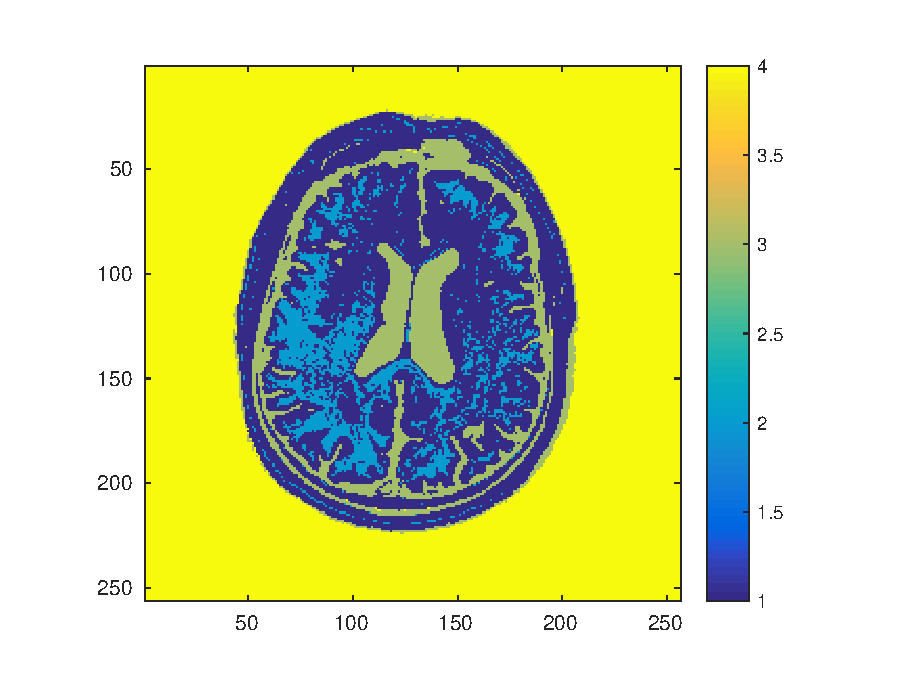
\includegraphics[width=\textwidth]{../4_NEW_IMAGE/NN_clasified.eps}
		\caption[]{\small Clasificación con Red Neuronal}
		\label{fig:new:nn}
	\end{subfigure}
	\quad
	\begin{subfigure}[b]{0.435\textwidth}
		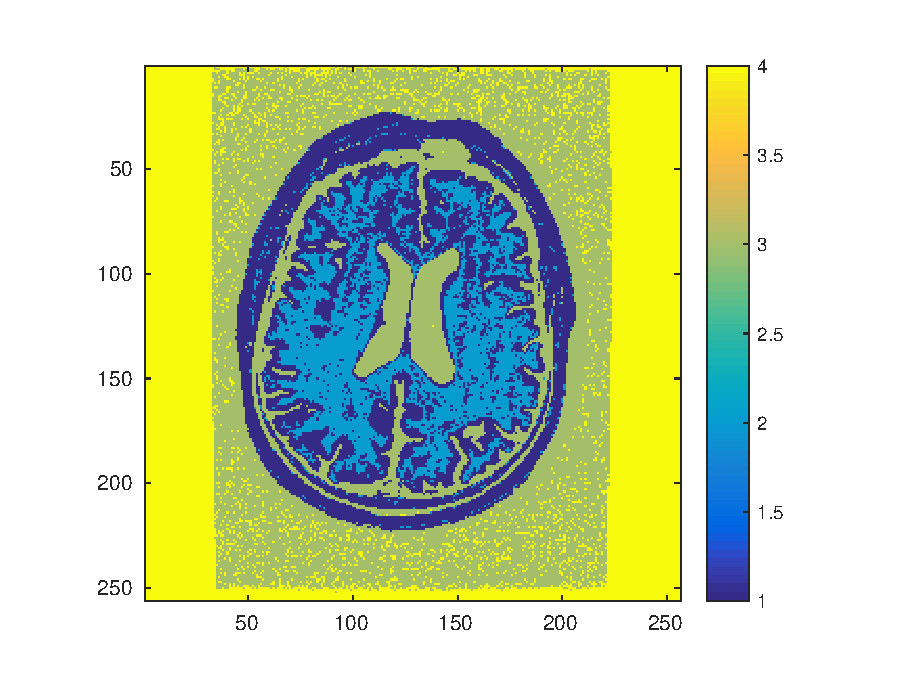
\includegraphics[width=\textwidth]{../4_NEW_IMAGE/Tree_clasified.eps}
		\caption[]{\small Clasificación con Árboles de Decisión}
		\label{fig:new:tree}
	\end{subfigure}
	\caption{Resultados de la clasificación con Red Neuronal y Árbol de decisión óptimos.}
	\label{fig:new}
\end{figure}

\end{document}
